\section{Results}
\label{sec:results}

\subsection{Answering Beyond Raw Retrieval}
\label{sec:res-main}

\begin{table*}[t]
\centering
\small
\setlength{\tabcolsep}{3.4pt}
\renewcommand{\arraystretch}{1.06}
\begin{tabular}{l|cc|cc|cc|cc}
\toprule
\multirow{2}{*}{\textbf{Method}} & \multicolumn{2}{c|}{\cellcolor{hME}\textbf{MemEye}} & \multicolumn{2}{c|}{\cellcolor{hML}\textbf{MemLens-32k}} & \multicolumn{2}{c|}{\cellcolor{hVM}\textbf{VisualMem}} & \multicolumn{2}{c}{\cellcolor{hCR}\textbf{CamRoll}} \\
 & \cellcolor{hME}Light & \cellcolor{hME}Strong & \cellcolor{hML}Light & \cellcolor{hML}Strong & \cellcolor{hVM}Light & \cellcolor{hVM}Strong & \cellcolor{hCR}Light & \cellcolor{hCR}Strong \\
\midrule
RAG@40 & .493 & .764 & .470 & .682 & .450 & .826 & .724 & .894 \\
Full context & .500 & \textbf{.810} & .446 & .691 & .454 & \textbf{.967} & -- & -- \\
\midrule
SimpleMem & .355 & .445 & .395 & .403 & .414 & .747 & .673 & .819 \\
Omni-SimpleMem & .311 & .373 & .384 & .421 & .425 & .746 & .614 & .718 \\
TeleMem & .339 & .398 & .200 & .159 & .368 & .703 & .639 & .744 \\
\midrule
V-Mem & .469 & .730 & .461 & .665 & .427 & .809 & .691 & .828 \\
MMA & .414 & .761 & .442 & .629 & .407 & .868 & .600 & .854 \\
\midrule
\oursrow \textbf{\vgs{} (ours)} & \textbf{.543}\,{\fontsize{6.2}{7}\selectfont$_{+10.1\%}$} & .793\,{\fontsize{6.2}{7}\selectfont$_{+3.8\%}$} & \textbf{.513}\,{\fontsize{6.2}{7}\selectfont$_{+9.1\%}$} & \textbf{.693}\,{\fontsize{6.2}{7}\selectfont$_{+1.6\%}$} & \textbf{.579}\,{\fontsize{6.2}{7}\selectfont$_{+28.8\%}$} & .921\,{\fontsize{6.2}{7}\selectfont$_{+11.5\%}$} & \textbf{.827}\,{\fontsize{6.2}{7}\selectfont$_{+14.2\%}$} & \textbf{.899}\,{\fontsize{6.2}{7}\selectfont$_{+0.6\%}$} \\
\bottomrule
\end{tabular}
\caption{\textbf{Main results.} Accuracy with the lightweight (Light) and the strong reader. Every method is evaluated on the same questions (371, 466, 696, and 1000) with the same readers, prompts, and judges. Subscripts give the relative change of \vgs{} over RAG@40; the best result per column is in bold. Costs are in Table~\ref{tab:cost}, and retrieval re-ranked by the selector model is compared in Table~\ref{tab:rerank}. Full context is not run on CamRoll, where a history holds about 800 photos.}
\label{tab:main}
\end{table*}


\paragraph{Lightweight reader.} \vgs{} is the most accurate method on all four benchmarks (Table~\ref{tab:main}). It improves over RAG@40 by 5.0 points on MemEye, 4.3 on MemLens, 12.9 on VisualMem, and 10.3 on CamRoll, and it also exceeds full-context reading, every memory system, and re-ranked retrieval (Table~\ref{tab:rerank}). The VisualMem and CamRoll gains are significant on their own. The MemEye and MemLens gains are individually at the margin ($p{=}0.055$ and $0.058$) and significant when pooled ($+4.6$ points, $p{=}0.007$) and on MemLens with 64k histories ($+5.8$; Appendix~\ref{app:robust}). Reading more does not help this reader: where it is run, full context stays within 2.4 points of RAG@40, and re-ranking adds at most 1.0 point except on VisualMem, at four to nine times the cost of RAG@40.

\paragraph{Strong reader.} \vgs{} is at least as accurate as RAG@40 on all four benchmarks, and its gain concentrates on VisualMem, where histories are long and most evidence lies outside the 40 most similar rounds. There \vgs{} reaches 0.921, against 0.826 for RAG@40 and 0.861 for re-ranked retrieval, and approaches full-context reading (0.967) at about a seventh of its cost. On MemEye, MemLens, and CamRoll, where the 40 most similar rounds already contain all the evidence for 91\%, 65\%, and 87\% of the questions, the strong reader leaves little room: RAG@40, re-ranked retrieval, and \vgs{} lie within 2.9 points of each other, \vgs{} does not differ significantly from RAG@40, and it costs less than re-ranked retrieval (Table~\ref{tab:rerank}). When the MemEye histories are enlarged to 1,171 and 4,088 rounds with other users' image chats, RAG@40 loses accuracy and the gain of \vgs{} grows to 6.6 and 4.8 points, both significant (Appendix~\ref{app:robust}).

\paragraph{Memory systems.} With the lightweight reader, RAG@40 is more accurate than every memory system on all four benchmarks. With the strong reader, the two systems that keep raw turns come closest to it: V-Mem trails RAG@40 by 1.7 to 6.6 points, and MMA matches it on MemEye, trails it by 5.4 and 4.0 points on MemLens and CamRoll, and exceeds it on VisualMem (0.868 against 0.826). The systems that write text records at ingestion fall furthest behind on MemEye and MemLens. \vgs{} is more accurate than every memory system in every column.

\subsection{Recovering Evidence That Similarity Misses}
\label{sec:res-select}

\begin{table}[t]
\centering
\small
\setlength{\tabcolsep}{4.2pt}
\renewcommand{\arraystretch}{1.06}
\begin{tabular}{l|c|cc|c}
\toprule
\rowcolor{hHead} & & \multicolumn{2}{c|}{\textbf{Cosine}} & \\
\rowcolor{hHead} \textbf{Benchmark} & Rds. & same size & top-40 & \textbf{\qss{}} \\
\midrule
MemEye & 7.2 & .523 & \textbf{.914} & .860 \\
\quad $\ge$4 gold rounds & 11.4 & .174 & \textbf{.791} & .744 \\
MemLens & 5.8 & .165 & \textbf{.648} & .373 \\
VisualMem & 6.0 & .254 & .454 & \textbf{.787} \\
CamRoll & 7.4 & .599 & .865 & \textbf{.868} \\
\bottomrule
\end{tabular}
\caption{\textbf{Selection without answering.} Full-set recall of the standard path's selection (\qss{}), of cosine retrieval with as many rounds as each \qss{} set (Rds., mean), and of top-40 retrieval. The second row covers the 86 MemEye questions with at least four gold rounds.}
\label{tab:select}
\end{table}

\begin{figure*}[t]
\centering
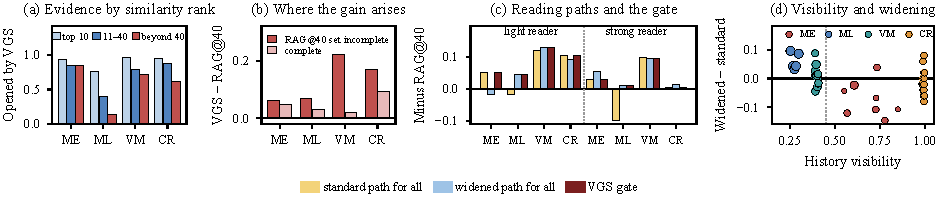
\includegraphics[width=\textwidth]{figures_polished/story_gate.pdf}
\caption{\textbf{How \vgs{} reads.} (a)~Share of gold rounds that \vgs{} opens, by their similarity rank; RAG@40 opens none beyond rank 40. (b)~Lightweight-reader gain over RAG@40 on questions for which the RAG@40 rounds miss evidence or contain all of it. (c)~One reading path for every history and the gate, relative to RAG@40. (d)~Lightweight-reader gain from widening against history visibility $H(h)$, with one point per history (per quintile of histories on MemLens); the dotted line marks $\tau$.}
\label{fig:vis}
\end{figure*}

The retrieval results show a gain before the reader answers. At matched per-question budgets, \qss{} recovers more complete evidence than cosine retrieval on all four benchmarks (Table~\ref{tab:select}). On MemEye, the gap is largest for questions with at least four gold rounds, where full-set recall is 0.744 against 0.174. On VisualMem, \qss{} finds the answer-bearing image for 0.787 of questions with 6.0 rounds, compared with 0.454 for top-40 retrieval. MemLens shows the limit of focused selection: \qss{} doubles the recall of same-size retrieval, but top-40 retrieval remains more complete. On CamRoll, \qss{} matches the full-set recall of top-40 retrieval (0.87) with 7.4 photos.

These differences arise where similarity ranks the evidence low (Figure~\ref{fig:vis}a). \vgs{} opens 85\% of the gold rounds outside the 40 most similar rounds on MemEye, 72\% on VisualMem, and 61\% on CamRoll, which RAG@40 never opens. Its gain is largest on the questions for which RAG@40 misses evidence (Figure~\ref{fig:vis}b). On VisualMem, where such questions are more than half of the benchmark, \vgs{} gains 22.1 points on them against 1.9 elsewhere, and on CamRoll 16.8 against 9.2. On MemEye and MemLens the contrast is smaller ($+6.2$ and $+6.7$ against $+4.9$ and $+3.0$), and on MemLens \vgs{} rarely opens low-ranked rounds; its gain there comes from the widened reading path (Section~\ref{sec:res-vis}).

\subsection{Index Reading and Coverage}
\label{sec:res-ablation}

\begin{table}[t]
\centering
\small
\setlength{\tabcolsep}{3.2pt}
\renewcommand{\arraystretch}{1.06}
\resizebox{\columnwidth}{!}{%
\begin{tabular}{lcccc}
\toprule
\textbf{Configuration} & \cellcolor{hME}\textbf{ME} & \cellcolor{hML}\textbf{ML} & \cellcolor{hVM}\textbf{VM} & \cellcolor{hCR}\textbf{CR} \\
\midrule
\oursrow \vgs{} (full) & .543 & .513 & .579 & .827 \\
\quad w/o widened path & .543\,{\fontsize{6.4}{7}\selectfont$+0.0$} & \cellcolor{dC}.453\,{\fontsize{6.4}{7}\selectfont$-6.0$} & \cellcolor{dA}.569\,{\fontsize{6.4}{7}\selectfont$-1.0$} & .827\,{\fontsize{6.4}{7}\selectfont$+0.0$} \\
\quad w/o standard path & \cellcolor{dC}.476\,{\fontsize{6.4}{7}\selectfont$-6.7$} & .513\,{\fontsize{6.4}{7}\selectfont$+0.0$} & .579\,{\fontsize{6.4}{7}\selectfont$+0.0$} & \cellcolor{dA}.815\,{\fontsize{6.4}{7}\selectfont$-1.2$} \\
\quad w/o whole index & \cellcolor{dB}.507\,{\fontsize{6.4}{7}\selectfont$-3.6$} & .513\,{\fontsize{6.4}{7}\selectfont$+0.0$} & \cellcolor{dC}.519\,{\fontsize{6.4}{7}\selectfont$-6.0$} & \cellcolor{dA}.816\,{\fontsize{6.4}{7}\selectfont$-1.1$} \\
\midrule
\oursrow \qss{}, 100-round pool & .507 & .453 & .522 & .816 \\
\quad w/o index reading & \cellcolor{dB}.465\,{\fontsize{6.4}{7}\selectfont$-4.2$} & \cellcolor{dC}.382\,{\fontsize{6.4}{7}\selectfont$-7.1$} & \cellcolor{dD}.392\,{\fontsize{6.4}{7}\selectfont$-12.9$} & \cellcolor{dC}.753\,{\fontsize{6.4}{7}\selectfont$-6.3$} \\
\quad w/o set output & .504\,{\fontsize{6.4}{7}\selectfont$-0.3$} & .453\,{\fontsize{6.4}{7}\selectfont$+0.0$} & .519\,{\fontsize{6.4}{7}\selectfont$-0.3$} & .829\,{\fontsize{6.4}{7}\selectfont$+1.3$} \\
\quad w/o adaptive size & .500\,{\fontsize{6.4}{7}\selectfont$-0.7$} & \cellcolor{dA}.431\,{\fontsize{6.4}{7}\selectfont$-2.1$} & .532\,{\fontsize{6.4}{7}\selectfont$+1.0$} & \cellcolor{dA}.799\,{\fontsize{6.4}{7}\selectfont$-1.7$} \\
\bottomrule
\end{tabular}}
\caption{\textbf{Ablations and selection controls.} Accuracy with the lightweight reader and point changes from the highlighted reference. Removing a reading path sends every history to the other one; \emph{w/o whole index} limits navigation to a 100-round cosine pool. On that pool, the selector is replaced by cosine retrieval of the same size (\emph{w/o index reading}), by its own ranking cut at the same size (\emph{w/o set output}), or by that ranking cut at eight rounds (\emph{w/o adaptive size}); full-set recall and the remaining rows are in Table~\ref{tab:ablation_full}. ME, ML, VM, and CR denote MemEye, MemLens, VisualMem, and CamRoll.}
\label{tab:ablation}
\end{table}


Global navigation improves selection even when the candidates and output budget are held fixed (Table~\ref{tab:ablation}). On a shared 100-round pool, \qss{} is more accurate than cosine retrieval of the same size on every benchmark, by 4.2 to 12.9 points. A ranking by the same model performs within 1.3 points of \qss{} when cut at the size that \qss{} chose and within 2.1 points when cut at eight rounds. Reading the index, rather than the output format, is therefore the source of the improvement. Table~\ref{tab:ablation_full} reports the corresponding evidence recall.

The index must also cover the whole history. Restricting navigation to the 100 rounds most similar to the question (\emph{w/o whole index}) lowers accuracy by 3.6 points on MemEye, 1.1 on CamRoll, and 6.0 on VisualMem, where this pool contains the complete evidence for only 60\% of the questions. The same limit bounds re-ranked retrieval end to end (Table~\ref{tab:rerank}): with the strong reader it is within 2 points of \vgs{} on MemEye and MemLens, where the pool is complete for 99\% and 100\% of the questions, and trails it by 6.0 points on VisualMem.

\subsection{Routing with Index Visibility}
\label{sec:res-vis}

Histories differ in how much of their content the index retains. Visibility ranges from 0.55 to 0.85 on the MemEye histories, whose messages are short, from 0.22 to 0.35 on MemLens, where evidence often lies beyond the first 200 characters of a message, and from 0.39 to 0.41 on VisualMem. For the lightweight reader, the better reading path follows this order (Figure~\ref{fig:vis}c,d): widening lowers accuracy on seven of the eight MemEye histories ($-6.7$ points overall), raises it on MemLens ($+6.0$), where longer index lines and notes each contribute about half of the gain (Appendix~\ref{app:vis}), and changes it little on VisualMem ($+1.0$). The gate selects the better path on all three, and also on the unseen CamRoll: its index lines show each photo's description in full (visibility 0.99), and the standard path is 1.2 points more accurate than widening.

For the strong reader, widening adds rounds without removing any, and it changes accuracy by $+2.6$ points on MemEye, $+10.9$ on MemLens, $-0.4$ on VisualMem, and $+0.8$ on CamRoll. The gate keeps MemEye and CamRoll on the standard path. For the strong reader this is a cost choice, not an accuracy choice: it gives up these 2.6 and 0.8 points and halves the cost on MemEye. Swapping the widened paths between the readers lowers accuracy in five of six cases (Table~\ref{tab:swap}), which supports widening by reader.

Visibility separates histories, not questions. Within a benchmark, a per-question estimate of visibility ranks the questions that gain from widening barely better than chance (AUC 0.47 to 0.63), while a per-question oracle would add 2 to 9 points (Table~\ref{tab:gate}).

\subsection{Cost}
\label{sec:res-cost}


Reading fewer raw rounds can offset the cost of navigation (Table~\ref{tab:cost}, Figure~\ref{fig:cost}). With a cached index, strong-reader \vgs{} costs \$5.5 per 1,000 questions on MemEye, against \$9.7 for RAG@40, and the two cost about the same on MemLens (\$13.8 and \$14.0). On the longer VisualMem and CamRoll histories, whose indexes hold tens of thousands of tokens, \vgs{} costs more than retrieval (\$6.6 and \$5.7 against \$1.0 and \$1.3 with the lightweight reader; \$23.1 and \$15.7 against \$8.8 and \$11.4 with the strong reader) and far less than full-context reading (\$154 on VisualMem). Median latency with the lightweight reader is 5.0~s on MemEye against 5.4~s for RAG@40 (Appendix~\ref{app:latency}).
